\chapter{Фермионные знаки и суперсимметрические компенсации}

\lectureoverview{Суперсимметрия связывает бозоны с фермионами, но понять, зачем нужна такая связь, легче еще до записи ее алгебры. Мы начнем с топологии вращений, сделаем знак фермионной волновой функции наблюдаемым посредством интерференции, выведем минус для замкнутой фермионной петли из антисимметрии при обмене, а затем используем противоположные знаки бозонных и фермионных петель, чтобы мотивировать компенсации вакуумной энергии и собственной энергии скаляра. Во второй половине ставятся вопросы о том, насколько сильно может быть нарушена суперсимметрия, как можно было бы обнаружить суперпартнеров и почему точная суперсимметрия стерла бы обычную оболочечную структуру атома.}

\section{До суперсимметрии: одна особенность вращений}

Суперсимметрия — это симметрия между фермионами и бозонами. Однако, прежде чем пытаться ее построить, полезно вспомнить, насколько по-разному эти два рода частиц ведут себя при вращениях. Сам этот вопрос начинается с топологического факта, который легко продемонстрировать и который, увидев однажды, удивительно трудно забыть.

Держите одну руку ладонью вверх и поверните кисть на \(2\pi\). Кисть вернется в исходную ориентацию, но рука явно не вернется к эквивалентной конфигурации: она перекручена. Продолжите еще на \(2\pi\), при необходимости двигая руку, и перекручивание можно будет снять. Следовательно, поворот на \(2\pi\) нельзя непрерывно деформировать в тождественное вращение при фиксированном окружении, тогда как поворот на \(4\pi\) можно. Эта демонстрация с рукой — доказательство размахиванием руками в самом буквальном смысле.

То же самое можно показать и без обращения к анатомии. Поместите шар в неподвижный ящик и прикрепите его к стенкам любым числом гибких, растяжимых, но неразрываемых нитей. Поверните шар один раз на \(2\pi\). Нити запутаются, и никакое движение одних только нитей не восстановит исходную конфигурацию. Поверните шар на суммарный угол \(4\pi\), и нити можно будет провести вокруг него так, что запутанность исчезнет. Стенки играют роль пространственной бесконечности: сравнение имеет смысл лишь потому, что граница не вращается вместе с шаром.

\begin{classroomqa}
\audiencequestion{Нельзя ли убрать запутанность, повернув ящик? \lecturetimestamp{00:02:53}}
\lecturerresponse{Это уже другая задача. Ящик представляет пространственную бесконечность и удерживается неподвижным. Мы сравниваем вращение объекта относительно окружения, а не совместное вращение объекта и окружения.}
\end{classroomqa}

\begin{classroomqa}
\audiencequestion{Почему бы просто не повернуть шар еще на \(2\pi\)? \lecturetimestamp{00:03:20}}
\lecturerresponse{Именно в этом и состоит различие между двумя случаями. Не поворачивая шар дальше, нельзя устранить запутанность, оставленную одним поворотом на \(2\pi\). После второго поворота, дающего в сумме \(4\pi\), это можно сделать.}
\end{classroomqa}

На современном языке теории групп группа вращений имеет два топологических класса замкнутых путей:
\begin{equation}
\pi_1\!\left(SO(3)\right)\cong \mathbb Z_2.
\end{equation}
Однократный обход нетривиален, но двукратный обход дает тривиальный класс.
Эквивалентно, \(SU(2)\) является двойным накрытием \(SO(3)\). Это геометрическая предыстория фермионного знака.

\editorialnote{Язык \(SO(3)\), \(SU(2)\) и фундаментальной группы делает топологию явной. Демонстрация с рукой и демонстрация с нитями геометрически устанавливают одно и то же двузначное поведение.}

\section{Что делает с квантовым состоянием поворот на \texorpdfstring{\(2\pi\)}{2 pi}}

Теперь зафиксируем положение частицы и сохраним только ее спиновое состояние, обозначаемое \(\ket{\psi}\). Частицы с целым спином — бозоны, а частицы с полуцелым спином — фермионы. Физическое вращение можно реализовать, поместив заряженную частицу со спином в сильное магнитное поле и вращая само поле, либо позволив спину прецессировать на нужный угол в фиксированном поле.

\begin{classroomqa}
\audiencequestion{Как в лаборатории реально повернуть спин электрона? \lecturetimestamp{00:05:26}}
\lecturerresponse{Рычагом служит магнитное поле. Можно вращать достаточно сильное поле так, чтобы спин следовал за ним, либо позволить спину прецессировать вокруг фиксированного поля. Браться за электрон руками — не самый конкурентоспособный экспериментальный метод.}
\end{classroomqa}

Предположим, что полный поворот на \(2\pi\) умножает состояние на фазовый множитель:
\begin{equation}
R(2\pi)\ket{\psi}=\xi\ket{\psi}.
\end{equation}
Двукратное выполнение этой операции дает
\begin{equation}
R(4\pi)\ket{\psi}=\xi^2\ket{\psi}.
\end{equation}
Поскольку путь на \(4\pi\) топологически тривиален, в этом сравнении он должен действовать как тождество. Поэтому
\begin{equation}
\xi^2=1,
\qquad
\xi=+1\ \hbox{or}\ -1.
\end{equation}
Бозонам соответствует знак плюс, а фермионам — минус:
\begin{align}
R(2\pi)\ket{\psi_B}&=+\ket{\psi_B},\\
R(2\pi)\ket{\psi_F}&=-\ket{\psi_F}.
\end{align}
Для состояния с определенным спином \(j\) это кратко записывается как
\begin{equation}
R(2\pi)=(-1)^{2j}.
\end{equation}
В расшифровке кратко говорится, что вторая возможность — умножение на \(2\pi\); из окружающего вывода и аргументации на доске ясно, что подразумевается множитель \(-1\).

Поначалу это кажется физически пустым. Если вся волновая функция меняет знак,
\begin{equation}
\Psi\longmapsto-\Psi,
\end{equation}
то вероятности не меняются, поскольку
\begin{equation}
(-\Psi)^*(-\Psi)=\Psi^*\Psi.
\end{equation}
Возьмите два ансамбля одинаково подготовленных электронов, поверните каждый член одного ансамбля на \(2\pi\), а другой ансамбль оставьте без изменения. Никакое измерение над отдельным электроном не может показать, из какого ансамбля он взят. Общая фаза ненаблюдаема.

\section{Сделать знак минус относительным}

Знак становится наблюдаемым, когда он накладывается на одну когерентную ветвь волновой функции, но не на другую. Пропускайте электроны по одному через двухпутевую установку. Не определяйте, по какому пути идет частица, потому что информация о пути разрушает интерференцию. Пусть верхняя и нижняя амплитуды равны \(\psi_1\) и \(\psi_2\), так что после рекомбинации состояние имеет вид
\begin{equation}
\Psi=\psi_1+\psi_2.
\end{equation}
Представьте, что каждая ветвь временно удерживается в магнитной области. Поверните только поле, связанное со второй ветвью, на \(2\pi\). Если частица — фермион, состояние становится
\begin{equation}
\Psi'=\psi_1-\psi_2.
\end{equation}
Это уже не общий знак. Относительная фаза превращает интерференционные максимумы в минимумы. Если два возвращающихся пакета зеркально симметричны относительно середины детектора, антисимметричная комбинация обращается в нуль в центре:
\begin{equation}
\Psi'(0)=\psi_1(0)-\psi_2(0)=0.
\end{equation}
Следовательно, в этой точке симметрии электрон никогда не обнаруживается. Если же повернуть обе ветви, получится \(-\psi_1-\psi_2=-\Psi\), что не имеет наблюдаемого эффекта.

В лекции подчеркивается относительный характер этого эксперимента. Поворот одной магнитной области относительно другой аналогичен повороту шара при неподвижном ящике. Совместный поворот обеих областей аналогичен совместному повороту шара и ящика. Относительный поворот на \(4\pi\) устраняет эффект, потому что фермионное состояние тогда возвращается со знаком плюс. Эксперимент был предложен Yakir Aharonov и Leonard Susskind в 1967 и позднее был реализован в интерферометрической форме, как мимоходом отмечается в лекции. Тот же принцип применим к электронам или заряженным ионам: сдвинутая интерференционная картина указывает на состояние с полуцелым спином, тогда как несдвинутая — на состояние с целым спином.

\begin{classroomqa}
\audiencequestion{Если относительное поле повернуть на \(4\pi\), вернется ли сдвинутая картина к исходной? \lecturetimestamp{00:12:21}}
\lecturerresponse{Да. Два изменения знака дают \(+1\), так что относительная фаза, отвечающая за перестановку максимумов и минимумов, исчезает.}
\end{classroomqa}

\begin{classroomqa}
\audiencequestion{Насколько буквально следует связывать нити в ящике с фермионом? \lecturetimestamp{00:13:43}}
\lecturerresponse{Это топологическая мнемоника, а не физические нити, прикрепленные к электрону. Бозон ведет себя так, как будто поворот на \(2\pi\) не оставляет памяти; фермион сохраняет именно ту память о знаке, которую и представляет нетривиальная запутанность.}
\end{classroomqa}

\begin{classroomqa}
\audiencequestion{Есть ли в двух магнитных областях два электрона, один в той, где поле повернули, а другой в той, где нет? \lecturetimestamp{00:14:29}}
\lecturerresponse{Нет. Имеется один электрон в когерентной пространственной суперпозиции. Он имеет амплитуду находиться в любой из ветвей, и установка не должна выявлять, какую ветвь он занимал. Поворот одной области меняет одну амплитуду относительно другой; поворот обеих меняет только общую фазу.}
\end{classroomqa}

Угол \(2\pi\) особый, потому что ориентация спина возвращается к самой себе, тогда как спинор приобретает знак. Произвольное относительное вращение меняет также ориентацию спина. Если два состояния двух путей возвращаются со спиновыми состояниями \(\ket{\chi_1}\) и \(\ket{\chi_2}\), интерференционный член пропорционален
\begin{equation}
\braket{\chi_1}{\chi_2}.
\end{equation}
Его модуль определяет видность интерференционных полос.\editorialnote{Формула с перекрытием спиновых состояний является стандартным дополнением к качественному обсуждению на лекции частичной и полной потери интерференции.} Ортогональные спиновые состояния несут полную информацию о том, по какому пути прошла частица, и не интерферируют.

\begin{classroomqa}
\audiencequestion{Что происходит, если измерить, в какой магнитной области находился электрон? \lecturetimestamp{00:18:03}}
\lecturerresponse{Интерференционная картина разрушается. Любая запись, различающая два пути, устраняет когерентное сложение их амплитуд.}
\end{classroomqa}

\begin{classroomqa}
\audiencequestion{Если все спины изначально направлены одинаково и измеряется конечный спин, меняет ли сама операция \(2\pi\) это направление? \lecturetimestamp{00:18:17}}
\lecturerresponse{Нет. После \(2\pi\) физическое направление спина остается тем же; лишь фермионная ветвь приобретает знак минус. Именно поэтому эта операция может изменять интерференцию, не оставляя иной ориентации спина в качестве маркера пути.}
\end{classroomqa}

\begin{classroomqa}
\audiencequestion{Что если поле повернуть только на \(\pi\), а не на \(2\pi\)? \lecturetimestamp{00:18:43}}
\lecturerresponse{Тогда направление спина меняется. Ветвь со спином вверх и ветвь со спином вниз различимы и не могут интерферировать. Промежуточные углы непрерывно уменьшают видимость; относительный поворот на \(180^\circ\) уничтожает ее полностью.}
\end{classroomqa}

\section{Обменная симметрия и знак замкнутой петли}

В обсуждении вращения был выделен один фермионный знак минус. Второй, тесно связанный с ним знак появляется при обмене тождественных частиц. Для двухчастичной волновой функции,
\begin{align}
P_{12}\Psi_B(1,2)&=+\Psi_B(1,2)=+\Psi_B(2,1),\\
P_{12}\Psi_F(1,2)&=-\Psi_F(1,2)=-\Psi_F(2,1).
\end{align}
бозонные состояния симметричны, а фермионные состояния антисимметричны.

\begin{figure}[htbp]
\centering
\includegraphics[width=0.74\textwidth]{lecture_02_figure_02.png}
\lectureframe{00:24:27}
\caption{Аргумент об обмене в обозначениях состояний. В кадре надежно читается только обозначение кета; уравнения антисимметрии набраны в тексте, а не приписаны неразборчивой меловой записи.}
\end{figure}

Теперь мы можем определить относительный знак замкнутой петли частицы, не вычисляя ее интеграл. Рассмотрим вакуумную диаграмму Фейнмана без внешних ножек. Ее можно представить либо как частицу, описывающую замкнутый путь в пространстве-времени, либо как пару частица-античастица, которая рождается, а позднее аннигилирует. Такая вакуумная диаграмма дает вклад в вакуумную амплитуду и тем самым в энергию вакуума.

Начнем с двух несвязанных копий петли. Несвязные диаграммы перемножаются, так что если одна петля имеет знак \(\sigma\), то пара имеет знак
\begin{equation}
\sigma^2=+1.
\end{equation}
Разрежем обе петли при одном и том же времени, скажем \(t=0\). На этом срезе имеются две тождественные частицы. Соедините их снова без обмена, и вернутся две отдельные петли. Если обменять две частицы перед повторным соединением, топология станет одной петлей. Обмен дает вклад \(+1\) для бозонов и \(-1\) для фермионов. Поскольку исходный знак двухпетлевой диаграммы был положительным, для получающихся однопетлевых диаграмм имеем
\begin{equation}
\begin{aligned}
\operatorname{sign}(\text{closed boson loop})&=+1,\\
\operatorname{sign}(\text{closed fermion loop})&=-1.
\end{aligned}
\end{equation}
В более общем случае диаграмма с \(L_F\) независимыми замкнутыми фермионными петлями несет множитель
\begin{equation}
(-1)^{L_F}.
\end{equation}
Лекция намеренно выводит это правило из обмена, а не ссылается на интегрирование по переменным Грассмана. Этот элементарный аргумент делает физическое происхождение знака наглядным.

\section{Противоположные знаки петель и энергия вакуума}

Бозонная вакуумная петля дает вклад в вакуумную энергию с одним знаком, тогда как фермионная петля входит с противоположным знаком. Это сразу наводит на мысль, потому что наблюдаемая плотность темной энергии чрезвычайно мала по сравнению с наивными оценками с обрезанием в квантовой теории поля. В лекции приводится пресловутое расхождение как примерно \(123\) порядков величины. Точное значение показателя зависит от того, какой ультрафиолетовый масштаб используется; существенный факт состоит в фантастическом несоответствии.

Величина петлевого вклада зависит не только от статистики. Она зависит от массы, заряда, кратности и взаимодействий. И все же, если бозон и фермион совпадают по всем существенным свойствам, их равные по модулю вклады могут сократиться:
\begin{equation}
\begin{gathered}
m_B=m_F,\qquad q_B=q_F,\qquad g_B=g_F,\\
\Delta\rho_{\mathrm{vac}}^{(B)}
+\Delta\rho_{\mathrm{vac}}^{(F)}=0.
\end{gathered}
\end{equation}
Это наблюдение не решает проблемы космологической постоянной. Оно лишь дает то, чего одни только обычные бозонные петли дать не могли: вклады противоположного знака. В точно ненарушенной глобально суперсимметричной теории сокращения вакуумной энергии при соответствующих предположениях действительно могут быть точными; после нарушения суперсимметрии наблюдаемое крошечное ненулевое значение остается необъясненным.\editorialnote{Это уточнение отделяет мотивацию лекции от гораздо более трудной проблемы космологической постоянной.}

Уже известно, что точное совпадение не описывает природу. Если бы у электрона был партнер со спином нуль и с той же массой и электрическим зарядом, электрон-позитронная аннигиляция через виртуальный фотон могла бы рождать пару таких частиц:
\begin{equation}
e^-e^+\longrightarrow\gamma^*
\longrightarrow\widetilde e^-\widetilde e^+.
\end{equation}
Вырожденный заряженный скаляр не ускользнул бы от обычных экспериментов на коллайдерах. Следовательно, бозон-фермионное отражение не может быть точной симметрией наблюдаемого спектра. Это отражение по типу частицы, а не отражение в физическом пространстве.

\section{Более непосредственная цель: собственная энергия скаляра}

Энергия вакуума — первый пример, но главная забота лекции состоит в радиационной нестабильности масс скаляров. Скаляр с изначально нулевой голой массой может получить поправку, квадратично чувствительную к обрезанию. Схематически,
\begin{equation}
\Delta m_H^2\sim \frac{g_B^2}{16\pi^2}\Lambda^2
\end{equation}
от бозонной петли. Для масс фермионов действует другая защита: когда безмассовый фермион обладает точной киральной симметрией, радиационные поправки не могут породить аддитивный массовый член. Это и был лево-правый аргумент предыдущей лекции.

Теперь представьте себе симметрию, достаточно жесткую, чтобы поместить скаляр и фермион в один мультиплет и согласовать их взаимодействия. Тогда появляется фермионная петля с противоположным знаком:
\begin{equation}
\Delta m_H^2
\sim
\frac{g_B^2-g_F^2}{16\pi^2}\Lambda^2+\cdots .
\end{equation}
Если суперсимметрия обеспечивает \(g_B=g_F\) и равенство масс, квадратичные члены сокращаются. Защита фермиона тем самым передается его бозонному партнеру. Это не просто численное совпадение между двумя диаграммами; симметрия должна обеспечивать сокращение во всех порядках и для всех допустимых взаимодействий.

Широкое сопоставление на доске показывает, как лекция переходит от изолированных петель к попарным петлевым поправкам для распространяющихся частиц.

\begin{figure}[htbp]
\centering
\includegraphics[width=0.79\textwidth]{lecture_02_figure_04.png}
\lectureframe{00:40:23}

\medskip
\begin{tikzpicture}[scale=0.9]
\draw (-4.2,0) circle (0.55);
\draw[dashed] (-2.4,0) circle (0.55);
\draw (0,0) -- (3.7,0);
\fill (1.85,0) circle (0.055);
\draw (1.85,0) -- (1.85,0.25);
\draw[dashed] (1.85,0.85) circle (0.6);
\end{tikzpicture}
\caption{Сопоставление на всей доске топологий обычных петель и петель партнеров. Набранный эскиз сохраняет только видимый топологический контраст; скрытые обозначения частиц в нем не проставляются.}
\end{figure}

После перерыва в аудитории аргумент начинается заново с того, что называется картиной нулевого порядка. Это не порядок в теории возмущений. Имеется в виду самое грубое, но полезное описание:
\begin{quote}
Для каждой частицы существует суперпартнер с противоположной статистикой. У каждого фермиона есть бозонный партнер, а у каждого бозона — фермионный партнер.
\end{quote}
В точной суперсимметричной теории партнеры были бы также вырождены, то есть имели бы одинаковую массу. Природа не вырождена таким образом. И все же, если массы не равны, но и не слишком далеки друг от друга, сокращение может остаться достаточно хорошим, чтобы не допустить взрывообразно большой скалярной поправки. При мягком нарушении суперсимметрии опасный масштаб схематически заменяется расщеплением суперпартнеров:
\begin{equation}
\Delta m_H^2\sim
\frac{g^2}{16\pi^2}\,\Delta m_{\mathrm{SUSY}}^2
\ln\!\frac{\Lambda^2}{\Delta m_{\mathrm{SUSY}}^2}
\end{equation}
с точностью до зависящих от модели коэффициентов.\editorialnote{Эта формула выражает качественное утверждение лекции о том, что несовершенное согласование масс оставляет остаточную поправку, контролируемую расщеплением; она не списана с доски.}

\section{Нарушенная суперсимметрия и экспериментальная ставка 2010 года}

На момент записи этой лекции в 2010 году не было обнаружено ни одного суперпартнера. Непосредственный вывод состоял в том, что эти партнеры, если они реальны, должны быть тяжелее известных частиц и недоступны для более ранних установок. Суперсимметричные модели также различают частицы, чьи массы возникают лишь после нарушения электрослабой симметрии, и состояния, которым разрешено иметь большие массы, не нарушающие симметрию. Лекция предлагает это как обоснование того, почему наблюдаемая половина суперсимметричного спектра может быть легкой, тогда как ненаблюдаемая половина тяжелее, при этом откровенно называя такую схему натяжкой. Сасскинд высказывает собственное ожидание, что суперпартнеры будут обнаружены, и тут же отмечает, что это догадка, а не результат.

Поэтому Большой адронный коллайдер занимал центральное место в ожиданиях, выраженных в лекции. От него ожидали поисков как бозона Хиггса, так и суперпартнеров. Эти утверждения нужно читать в их контексте 2010 года: лекция излагает экспериментальную ставку до открытия бозона Хиггса и до последующих результатов поисков на Большом адронном коллайдере.

Почему суперпартнер, постулируемый из соображений естественности, не должен находиться на планковском масштабе? Потому что тогда он не выполнил бы возложенную на него задачу. Если массы бозона и фермиона различаются колоссально, их петлевые интегралы перестают сокращаться выше меньшей из двух масс. Остаточная скалярная поправка определяется примерно большим расщеплением, а не слабым масштабом. Суперсимметрия на сколь угодно далеком масштабе остается математической симметрией, но уже не дает убедительного объяснения легкого хиггсовского сектора.

Лекция переводит это в характерное для своей эпохи ожидание, что соответствующие расщепления должны лежать примерно в пределах нескольких сотен ГэВ и, следовательно, в области досягаемости LHC. Эта численная оценка исторически обусловлена и зависит от модели; важнее логическая цепочка:
\begin{equation}
\begin{gathered}
\text{Higgs protection}\\
\Downarrow\\
\text{effective boson--fermion cancellation}\\
\Downarrow\\
\Delta m_{\mathrm{SUSY}}\ \text{not too large}.
\end{gathered}
\end{equation}

\begin{classroomqa}
\audiencequestion{Могли бы все фермионные вклады просто суммарно компенсировать все бозонные вклады, без соответствия партнёров один к одному? \lecturetimestamp{00:45:01}}
\lecturerresponse{Численно они могли бы сократиться, но это было бы случайное сокращение, столь же тонко подстроенное, как и исходная проблема. Суперсимметричное предложение сильнее: разумные постулаты навязывают согласованные вклады, а нарушенная суперсимметрия объясняет, почему массы совпадают лишь приблизительно. Энергия вакуума служила иллюстрацией; непосредственная забота здесь — собственная энергия Хиггса.}
\end{classroomqa}

\begin{classroomqa}
\audiencequestion{Не предполагает ли уже утверждение, что суммарная компенсация неестественна, редукционистский способ организации теории? \lecturetimestamp{00:47:51}}
\lecturerresponse{Это справедливое возражение. Ни у кого нет окончательного определения естественности, и поиск отчасти сводится к тому, чтобы нащупать убедительное объяснение. Суперсимметрия и спонтанное нарушение суперсимметрии дают известные математические рамки, которые могут навязать желаемую структуру. Нерешёнными остаются вопросы, использует ли природа эту схему и является ли она единственной.}
\end{classroomqa}

\section{Прямое рождение, виртуальные эффекты и цепочки распадов}

Тяжёлую частицу не обязательно рождать на массовой оболочке, чтобы она влияла на эксперимент. Она может виртуально возникать внутри петли и слегка изменять обычную амплитуду электрон-позитронного рассеяния. Поэтому прецизионные электрослабые измерения накладывают ограничения на суперпартнёров даже тогда, когда энергия в системе центра масс ниже порога их прямого парного рождения
\begin{equation}
\sqrt{s}<2m_{\widetilde p}.
\end{equation}
Согласно оценке, данной в лекции в 2010 году, прецизионные данные уже сужали пространство параметров суперсимметрии, но ещё не исключали её.

\begin{classroomqa}
\audiencequestion{Можно ли было бы косвенно судить о суперпартнёрах, как раньше ограничивали тяжёлые частицы по точным скоростям рождения ещё до прямого наблюдения? \lecturetimestamp{00:49:01}}
\lecturerresponse{Да. Виртуальная петля суперпартнёра слегка изменяет обычную амплитуду, так что задача становится вопросом высокоточной электрослабой феноменологии, а не прямого рождения. Особенно полезным был бы чистый электрон-позитронный коллайдер с достаточно большой энергией. Столкновения протонов устроены более грязно, потому что протон — составное состояние кварков и глюонов; на самом деле сталкиваются флуктуирующие составляющие, а не две элементарные частицы с точно известными начальными условиями.}
\end{classroomqa}

Один из студентов спрашивает, нельзя ли пустить реакцию в обратную сторону, начиная с большого числа суперчастиц. Препятствие состоит не в симметрии обращения времени, а в доступности таких частиц. Тяжёлые суперпартнёры сначала нужно создать, и ожидается, что большинство из них быстро распадётся на более лёгкие состояния.

\begin{classroomqa}
\audiencequestion{Если бы во Вселенной было много суперчастиц, могли бы две из них столкнуться и превратиться в обычные частицы? \lecturetimestamp{00:53:43}}
\lecturerresponse{В принципе у соответствующих реакций есть обратные каналы, но не ожидается, что тяжёлые суперпартнёры будут свободно и в большом количестве сохраняться в природе. Они распадаются в состояния с меньшей энергией, поэтому эксперимент сначала должен обеспечить достаточно большую энергию столкновения, чтобы их создать.}
\end{classroomqa}

Это поднимает вопрос о тёмной материи. Во многих суперсимметричных моделях дискретное правило отбора не позволяет конечному суперпартнёру в цепочке распада полностью исчезнуть. Тогда каждый более тяжёлый суперпартнёр каскадно переходит к самому лёгкому суперпартнёру, или LSP. Если LSP электрически нейтрален, он может быть стабильным и трудным для обнаружения, что делает его возможным кандидатом на роль тёмной материи. В одном месте стенограмма в этом обмене репликами говорит «тёмная энергия», но вопрос аудитории и описание частицы недвусмысленно относятся к тёмной материи.

\begin{classroomqa}
\audiencequestion{Не противоречит ли быстрый распад суперпартнёров предположению, что суперпартнёр мог бы быть тёмной материей? \lecturetimestamp{00:54:53}}
\lecturerresponse{Нет. Большинство суперпартнёров может распадаться, тогда как самый лёгкий остаётся стабильным в моделях, где в конце каждой цепочки распада должен оставаться суперпартнёр. Электрический заряд обычно создаёт дополнительные феноменологические трудности, так что жизнеспособный LSP, вероятно, нейтрален. В принципе он обнаружим, но не оставлял бы очевидного ионизирующего трека, как заряженный селектрон.}
\end{classroomqa}

\section{Совпадение означает совпадение констант связи}

Одного лишь совпадения масс недостаточно. Сравните вакуумную петлю электрона с петлёй селектрона. Их противоположная статистика даёт противоположные знаки, но равенство модулей требует равенства масс. Теперь присоединим два внешних фотона. Коэффициенты содержат также электрические константы связи, так что компенсация требует равенства зарядов:
\begin{equation}
\begin{gathered}
q_{\widetilde e}=q_e,\\
\mathcal A_{\mathrm{loop}}^{(e)}
+\mathcal A_{\mathrm{loop}}^{(\widetilde e)}=0,\\
\text{provided the full couplings match.}
\end{gathered}
\end{equation}
Несовпадение на любом уровне оставляет нескомпенсированный расходящийся член. Суперсимметрия ценна тем, что связывает не только названия и спины, но и взаимодействия.

\begin{figure}[H]
\centering
\includegraphics[width=0.66\textwidth]{lecture_02_figure_05.png}
\lectureframe{00:57:15}

\medskip
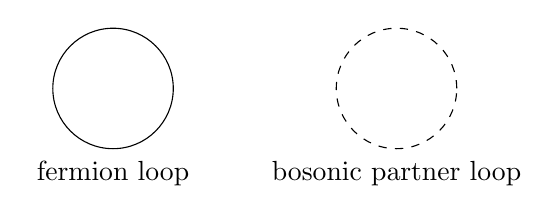
\begin{tikzpicture}[scale=0.9]
\draw (-2.0,0) circle (0.85);
\draw[dashed] (2.0,0) circle (0.85);
\node at (-2.0,-1.2) {fermion loop};
\node at (2.0,-1.2) {bosonic partner loop};
\end{tikzpicture}
\caption{Сравнение сплошной и штриховой петель в рассуждении о согласовании зарядов. Обрезанные внешние метки не восстановлены, поскольку одна лишь рамка не определяет все присоединения.}
\end{figure}

\begin{classroomqa}
\audiencequestion{Могли ли суперпартнёры ускользнуть от обнаружения просто потому, что их константы связи различны? \lecturetimestamp{00:56:23}}
\lecturerresponse{Нет, если одни и те же диаграммы должны сокращаться. Добавление фотонных взаимодействий проверяет электрический заряд каждой линии. Неравные константы связи дают разные численные петлевые множители и восстанавливают большой остаток. Симметрия должна согласовывать соответствующие заряды и взаимодействия.}
\end{classroomqa}

\begin{classroomqa}
\audiencequestion{Должен ли суперпартнёр фотона тоже быть безмассовым? \lecturetimestamp{00:58:01}}
\lecturerresponse{В точной суперсимметричной теории он был бы безмассовым, поскольку был бы вырожден по массе с фотоном. Наблюдаемый мир не является в точности суперсимметричным, так что физическое фотино-подобное состояние не обязано иметь ту же массу, что и фотон.}
\end{classroomqa}

\section{Словарь суперпартнёров}

Правила наименования не слишком изящны, но полезны. Бозону соответствует фермионный партнёр, название которого часто оканчивается на \emph{-ino}: фотон и фотино, \(W\) и вино, \(Z\) и зино, глюон и глюино, Хиггс и хиггсино, гравитон и гравитино. Обычному фермиону соответствует бозонный партнёр, название которого обычно начинается с \emph{s-}: электрон и селектрон, кварк и скварк.

\begin{center}
\begin{tabular}{@{}>{\raggedright\arraybackslash}p{0.40\linewidth}>{\raggedright\arraybackslash}p{0.52\linewidth}@{}}
\toprule
обычное состояние & суперпартнёр и изменение спина\\
\midrule
скалярный Хиггс, \(j=0\) & хиггсино, \(j=\tfrac12\); \(\Delta j=+\tfrac12\)\\
калибровочный бозон, \(j=1\) & гаугино, \(j=\tfrac12\); \(\Delta j=-\tfrac12\)\\
фермион вещества, \(j=\tfrac12\) & сфермион, \(j=0\); \(\Delta j=-\tfrac12\)\\
гравитон, \(j=2\) & гравитино, \(j=\tfrac32\); \(\Delta j=-\tfrac12\)\\
\bottomrule
\end{tabular}
\end{center}

Общее соотношение таково: члены супермультиплета различаются на половину единицы спина:
\begin{equation}
\Delta j=\frac12.
\end{equation}
В грубых примерах из лекции фермион вещества со спином \(\tfrac12\) образует пару со скаляром, а калибровочный бозон со спином единица — с гаугино со спином \(\tfrac12\). В полной взаимодействующей модели состояния после нарушения симметрии могут смешиваться, так что физические массовые собственные состояния не обязаны сохранять эти простейшие названия.

\begin{classroomqa}
\audiencequestion{Могут ли все новые скалярные партнёры сами испытать спонтанное нарушение симметрии? \lecturetimestamp{01:01:27}}
\lecturerresponse{Скалярные поля могут приобретать средние значения, но произвольное дополнительное нарушение симметрии было бы феноменологически катастрофичным. Жизнеспособная суперсимметричная модель должна так устроить свой скалярный потенциал, чтобы цвет, электрический заряд и другие необходимые симметрии не нарушались неправильным образом.}
\end{classroomqa}

\begin{classroomqa}
\audiencequestion{Есть ли у хиггсино особые взаимодействия, соответствующие квартическому члену Хиггса? \lecturetimestamp{01:02:19}}
\lecturerresponse{Суперсимметрия согласует взаимодействия так же, как и частицы. Это соотношение не получается простым наивным заменением каждой линии Хиггса линией хиггсино, но скалярное квартическое взаимодействие и соответствующие фермионные и вспомогательные взаимодействия входят в одну ограниченную структуру. Эти детали в лекции ещё не были разработаны.}
\end{classroomqa}

\begin{classroomqa}
\audiencequestion{Есть ли у теоремы о различии между поворотами на \(2\pi\) и \(4\pi\) аналоги в других размерностях? \lecturetimestamp{01:03:07}}
\lecturerresponse{Да, но размерность меняет возможности. В двух пространственных измерениях пути обмена могут обвиваться друг вокруг друга, что допускает энионы, у которых фазы обмена более общие, чем бозонное \(+1\) и фермионное \(-1\). Такие возбуждения встречаются в системах конденсированного вещества, но они лежат вне маршрута нынешнего курса.}
\end{classroomqa}

\section{Почему точная суперсимметрия уничтожила бы химию}

Наконец, спросим, каким был бы мир с точной суперсимметрией. Точность здесь означает равные массы и согласованные взаимодействия для каждой пары частица—суперпартнёр. У электрона был бы бозонный селектрон с той же массой и тем же электрическим зарядом, а у безмассового фотона было бы безмассовое фермионное фотино:
\begin{equation}
m_{\widetilde e}=m_e,
\qquad
q_{\widetilde e}=q_e,
\qquad
m_{\widetilde\gamma}=m_\gamma=0.
\end{equation}

Знакомая периодическая структура химии зависит от статистики Ферми. У водорода на самой низкой орбитали находится один электрон. Гелий вмещает там два электрона, поскольку их спиновые состояния различны. Третий электрон лития должен занимать более высокую орбиталь: принцип запрета Паули не позволяет трём одинаковым электронам занимать одно и то же одночастичное состояние. Этот внешний электрон имеет большую энергию и предпочёл бы перейти на более внутреннюю орбиталь, обычно испуская фотон, но заполненные нижние состояния блокируют переход.

Точная суперсимметрия открывает другой канал:
\begin{equation}
e^-_{\mathrm{outer}}
\longrightarrow
\widetilde e^-_{\mathrm{inner}}
+
\widetilde\gamma .
\end{equation}
Исходный электрон и испущенное фотино — фермионы, тогда как остающийся селектрон — бозон. Поскольку селектроны подчиняются статистике Бозе, а не Ферми, конечному селектрону не запрещено занять уже занятую нижнюю орбиталь. Поэтому валентный электрон может превратиться в селектрон и перейти на более внутреннюю орбиталь.

\begin{figure}[H]
\centering
\includegraphics[width=0.62\textwidth]{lecture_02_figure_06.png}
\lectureframe{01:09:18}

\medskip
\begin{tikzpicture}[scale=0.9]
\fill (0,0) circle (0.075);
\draw (0,0) circle (0.72);
\draw (0,0) circle (1.45);
\draw[-{Latex[length=2.2mm]}] (1.42,0.2) .. controls (1.2,0.52) and (0.92,0.42) .. (0.72,0.1);
\draw[decorate,decoration={snake,amplitude=1.4pt,segment length=7pt},-{Latex[length=2.2mm]}]
  (1.58,0) -- (3.55,0);
\node[above] at (2.7,0.12) {$\widetilde\gamma$};
\node[below] at (0,-1.65) {selectron drops to a lower orbital};
\end{tikzpicture}
\caption{Атомный переход, используемый для демонстрации того, почему точная суперсимметрия изменила бы химию. Исходящая волнистая линия показана; её отождествление с фотино следует из расшифровки лекции.}
\end{figure}

Этот вывод не ограничивается литиеподобным атомом. В большом атоме именно валентные электроны создают химическое разнообразие. Если они могут многократно превращаться в бозонные селектроны, то будут скапливаться в наиболее низкой по энергии доступной области, вместо того чтобы заполнять оболочки. В результате возникла бы концентрированная бозонная популяция вблизи ядра, а не привычная архитектура валентных орбиталей. Молекулы, построенные на направленных связях и частично заполненных оболочках, не сохранились бы в узнаваемом виде. В лекции гипотетический потомок лития назван \emph{slithium}, но за этой шуткой стоит серьёзный вывод: точная суперсимметрия породила бы вещество, отличное от вещества обычной химии и, следовательно, обычной биологии.

\begin{classroomqa}
\audiencequestion{Может ли переход электрона в селектрон иметь настолько малую константу связи, что обычные атомы сохранились бы? \lecturetimestamp{01:10:23}}
\lecturerresponse{Нет, не в рассматриваемой здесь точной теории. Суперсимметрия связывает этот переход с электромагнитным взаимодействием, так что его константа связи определяется электрическим зарядом, а не может быть произвольно выбрана сколь угодно малой. В лекции для литиеподобного атома приводится грубая оценка времени жизни порядка микросекунды — не как точный расчёт, а чтобы подчеркнуть, что распад был бы быстрым.}
\end{classroomqa}

Поэтому уже из свойств обычного вещества, совершенно независимо от поисков на коллайдерах, мы знаем, что при низких энергиях суперсимметрия не может быть точной. Разрыв между массами частиц и суперпартнёров огромен по сравнению с атомными или протонными масштабами, даже если по сравнению с масштабом великого объединения или планковским масштабом он был бы ничтожным.

\begin{classroomqa}
\audiencequestion{Почему же тогда суперсимметрия нарушена? \lecturetimestamp{01:11:19}}
\lecturerresponse{В лекции предлагается минимальное селекционное соображение: если бы она не была нарушена, не нашлось бы наблюдателей, построенных из обычной химии, чтобы задать этот вопрос. Это не заменяет динамической теории нарушения суперсимметрии. Оно объясняет лишь, почему мир низких энергий с точной суперсимметрией не мог бы быть нашим.}
\end{classroomqa}

Нарушение суперсимметрии математически возможно и во многих построениях довольно типично, хотя получить реалистическое нарушение отнюдь не автоматически. Напротив, точно суперсимметричные квантовые теории поля обладают настолько особой структурой, что некоторые из них можно анализировать гораздо глубже, чем теории общего вида. Они служат и кандидатами на роль организующего принципа физики частиц, и необычайно мощными математическими лабораториями. В следующей лекции акцент смещается от этой физической мотивации к более подробному рассмотрению этой структуры.

\section{Нить рассуждения}

Путь к суперсимметрии был намеренно непрямым:
\begin{enumerate}
\item Пространственное вращение на \(2\pi\) относится к нетривиальному топологическому классу, тогда как вращение на \(4\pi\) непрерывно деформируется в тождественное преобразование.
\item Состояние фермиона при вращении на \(2\pi\) приобретает знак минус, и эксперимент с двумя путями делает этот знак наблюдаемым, когда он является относительным, а не глобальным.
\item Фермионная антисимметрия при обмене даёт каждой замкнутой фермионной петле дополнительный знак минус по сравнению с бозонной петлёй.
\item Противоположные знаки петель допускают обусловленные симметрией сокращения вкладов в энергию вакуума и собственную энергию скаляра, когда массы и константы связи совпадают.
\item Точное совпадение в природе отсутствует. Если суперсимметрия защищает сектор Хиггса, её нарушение не может сделать соответствующих партнёров сколь угодно тяжёлыми.
\item Точная суперсимметрия при низких энергиях позволила бы электронам превращаться в бозонные селектроны и разрушила бы оболочечную структуру, от которой зависит обычная химия.
\end{enumerate}

Итак, суперсимметрия одновременно привлекательна и невозможна в своей наивной точной форме по одной и той же причине: она тесно связывает бозоны и фермионы. Эта тесная связь может укрощать опасные квантовые поправки, но если бы она без нарушения сохранялась и в атомной физике, мир перестал бы быть похожим на тот, что нас окружает.
